\chapter{Project plan}
\section*{Background \& Motivation}
Offshore wind turbines operate in harsh and highly dynamic environments. The structural integrity of bolted joints is critical for ensuring operational safety and minimizing maintenance costs. Loss of preload in bolted joints can lead to fatigue damage, misalignment, or catastrophic failure. The inability to detect gradual preload loss is a key limitation of current inspection methods, which rely heavily on periodic manual inspection and torque verification. This approach is not only discontinuous and costly, but also particularly problematic for offshore applications.

A compact, low-power, wireless, long-term strain monitoring system is required for permanent installation on critical bolted joints. This need is addressed by developing a complete integrated system and demonstrating a fully functional prototype suitable for long-term offshore deployment.

\section*{Literature \& Related Work}
Prior research demonstrates that wireless strain sensing for long-term monitoring applications is technically feasible, but no existing solution simultaneously satisfies the specific constraints of this project.

Integrated and compact strain sensing systems with wireless data transmission have been extensively documented in the literature \cite{SHM_bog, wireless_strain_sensor}. Similarly, the concept of long-term structural health monitoring has been widely investigated, particularly within offshore applications \cite{offshore_sensor_solutions, WindTurbineStrainSensor, StrainBand}.
Despite these advances, commercially available solutions based on conventional metal foil strain gauges require substantial signal conditioning, including amplification and noise mitigation \cite{MetalFoilStrain}. This increases system complexity, power consumption, and physical footprint, thereby limiting miniaturization and long-term autonomous operation.
Cost considerations further complicate deployment in large-scale structural applications. In offshore wind turbines, the number of critical bolted joints can reach several thousands per structure \cite{6000bolts}, making low unit cost a decisive factor for practical implementation.

To address these limitations, this thesis will explore the development of 3D-printed strain sensors \cite{G.O.A.T, 3DprintStrain, 3DprintWheatstoneStrain}, enabling rapid prototyping, geometric optimization, low-cost fabrication, and low-power integration.
This project aims to integrate ultra-low-power, small form factor, and full environmental sealing to solve the specific problem of long-term preload monitoring of bolted joints under offshore conditions. In this way, the project builds on existing approaches while extending them into a highly constrained and application-specific context.


\section*{Problem Statement}
The project aims to answer the following main research question:\\
How can a compact, wireless, strain sensor system be designed and validated to reliably measure $\le$800 µstrain elongated deformation on an M48 steel nut under offshore environmental conditions for more than 10 years of operation?

\pagebreak
\textbf{Sub-questions:}
\begin{itemize}
    \item[-] How can 3D printed sensor characteristics be optimized for accurate strain transfer and sensitivity?
    \item[-] How can encapsulation ensure oil, grease, and water resistance while maintaining strain transfer?
    \item[-] How can a strain measurement system be implemented within a 30 × 30 mm metallic surface?
    \item[-] How can a complete system be integrated to acquire data across numerous bolted joints in a wind turbine?
    \item[-] How can ultra-low-power electronics enable >10-year battery lifetime?
    \item[-] How can sensor performance in -20\textdegree C to +50\textdegree C be evaluated?
\end{itemize}

\section*{Work Breakdown Structure}
This project is conducted by a group of three, and the project management therefore has to be carefully considered to avoid inactivity. To reflect the 3 × 30 ECTS workload and ensure parallelization while maximizing resource utilization, the project is divided into interconnected work packages, as shown in \cref{fig:wbs}.

\definecolor{IBM1}{HTML}{648fff}%blå
\definecolor{IBM2}{HTML}{785ef0}%blå
\definecolor{IBM3}{HTML}{dc267f}%rød
\definecolor{IBM4}{HTML}{fe6100}%orange
\definecolor{IBM5}{HTML}{ffb000}%gul
\definecolor{IBM6}{HTML}{d55e00}%orange-brun
\definecolor{IBM7}{HTML}{cc79a7}%lilla
\definecolor{IBM8}{HTML}{0072b2}%blågrøn
\definecolor{IBM9}{HTML}{f0e442}%gul
\definecolor{IBM10}{HTML}{009e73}%grøn

\begin{figure}[htbp]
    \centering
    \resizebox{\textwidth}{!}{%
    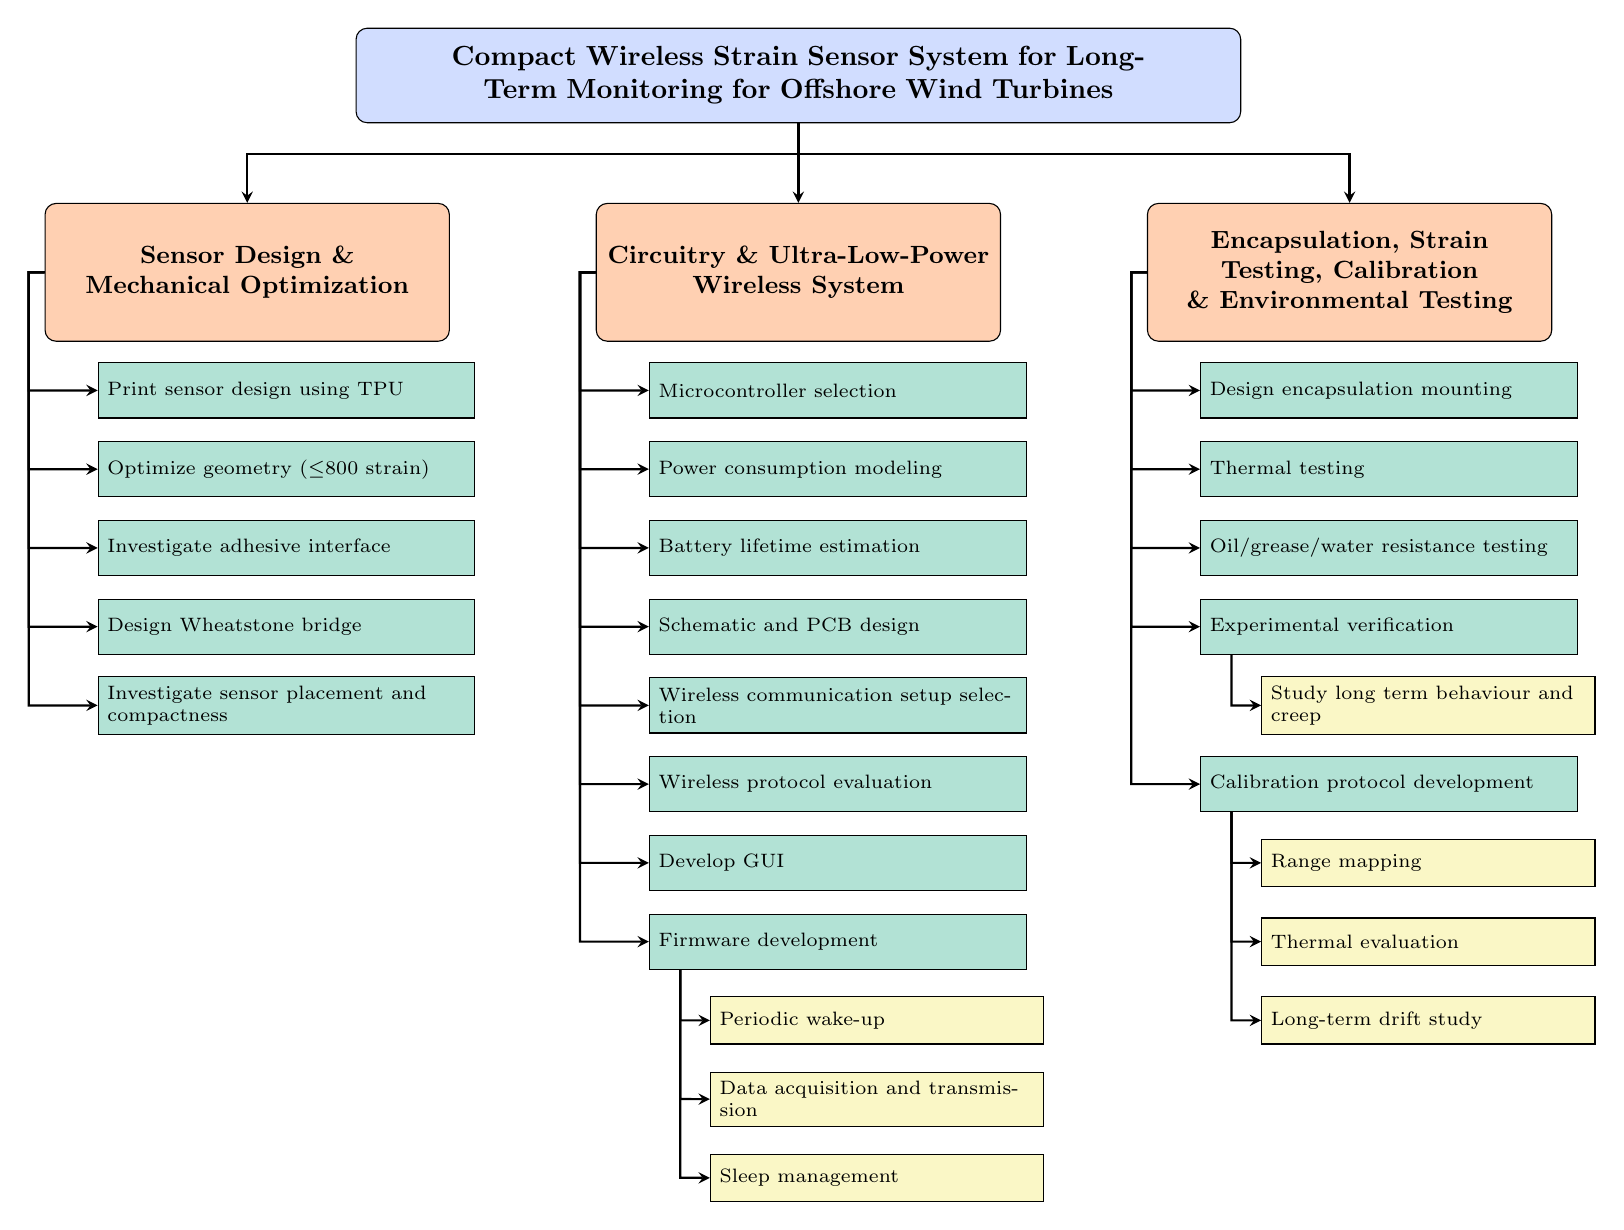
\begin{tikzpicture}[
        box/.style={rectangle, draw, fill=IBM1!30, text width=11cm, align=center, minimum height=1.2cm, rounded corners},
        wp/.style={rectangle, draw, fill=IBM4!30, text width=4.9cm, align=center, minimum height=1.75cm, rounded corners, font=\small\bfseries},
        task/.style={rectangle, draw, fill=IBM10!30, text width=4.55cm, align=left, minimum height=0.7cm, font=\scriptsize},
        subtask/.style={rectangle, draw, fill=IBM9!30, text width=4cm, align=left, minimum height=0.6cm, font=\scriptsize},
        arrow/.style={->, >=stealth, thick}
    ]

    \node[box] (root) at (0,0) {\textbf{Compact Wireless Strain Sensor System for Long-Term Monitoring for Offshore Wind Turbines}};
    
    \node[wp] (wp1) at (-7,-2.5) {Sensor Design \&\\ Mechanical Optimization};
    \node[wp] (wp2) at (0,-2.5) {Circuitry \& Ultra-Low-Power\\Wireless System};
    \node[wp] (wp3) at (7,-2.5) {Encapsulation, Strain\\Testing, Calibration\\\& Environmental Testing};

    % WP1
    \node[task] (wp1t1) at (-6.5,-4) {Print sensor design using TPU};
    \node[task] (wp1t2) at (-6.5,-5) {Optimize geometry ($\le$800 $\upmu$strain)};
    \node[task] (wp1t3) at (-6.5,-6) {Investigate adhesive interface};
    \node[task] (wp1t4) at (-6.5,-7) {Design Wheatstone bridge};
    \node[task] (wp1t5) at (-6.5,-8) {Investigate sensor placement and compactness};
    
    % WP2
    \node[task] (wp2t1) at (0.5,-4) {Microcontroller selection};
    \node[task] (wp2t2) at (0.5,-5) {Power consumption modeling};
    \node[task] (wp2t3) at (0.5,-6) {Battery lifetime estimation};
    \node[task] (wp2t4) at (0.5,-7) {Schematic and PCB design};
    \node[task] (wp2t5) at (0.5,-8) {Wireless communication setup selection};
    \node[task] (wp2t6) at (0.5,-9) {Wireless protocol evaluation};
    \node[task] (wp2t7) at (0.5,-10) {Develop GUI};
    \node[task] (wp2t8) at (0.5,-11) {Firmware development};
    \node[subtask] (wp2t8a) at (1,-12) {Periodic wake-up};
    \node[subtask] (wp2t8b) at (1,-13) {Data acquisition and transmission};
    \node[subtask] (wp2t8c) at (1,-14) {Sleep management};

    % WP3
    \node[task] (wp3t1) at (7.5,-4) {Design encapsulation mounting};
    \node[task] (wp3t2) at (7.5,-5) {Thermal testing};
    \node[task] (wp3t3) at (7.5,-6) {Oil/grease/water resistance testing};
    \node[task] (wp3t4) at (7.5,-7) {Experimental verification};
    \node[subtask] (wp3t4a) at (8,-8) {Study long term behaviour and creep};
    \node[task] (wp3t5) at (7.5,-9) {Calibration protocol development};
    \node[subtask] (wp3t5a) at (8,-10) {Range mapping};
    \node[subtask] (wp3t5b) at (8,-11) {Thermal evaluation};
    \node[subtask] (wp3t5c) at (8,-12) {Long-term drift study};

    % Arrows
    \draw[arrow] (root) --++ (0,-1) -- (-7,-1) -- (wp1);
    \draw[arrow] (root) --++ (0,-1) -- (wp2);
    \draw[arrow] (root) --++ (0,-1) -- (7,-1) -- (wp3);

    \draw[arrow] (wp1.west) --++ (-0.2,0) --++ (0,-1.5) -- (wp1t1.west);
    \draw[arrow] (wp1.west) --++ (-0.2,0) --++ (0,-2.5) -- (wp1t2.west);
    \draw[arrow] (wp1.west) --++ (-0.2,0) --++ (0,-3.5) -- (wp1t3.west);
    \draw[arrow] (wp1.west) --++ (-0.2,0) --++ (0,-4.5) -- (wp1t4.west);
    \draw[arrow] (wp1.west) --++ (-0.2,0) --++ (0,-5.5) -- (wp1t5.west);

    \draw[arrow] (wp2.west) --++ (-0.2,0) --++ (0,-1.5) -- (wp2t1.west);
    \draw[arrow] (wp2.west) --++ (-0.2,0) --++ (0,-2.5) -- (wp2t2.west);
    \draw[arrow] (wp2.west) --++ (-0.2,0) --++ (0,-3.5) -- (wp2t3.west);
    \draw[arrow] (wp2.west) --++ (-0.2,0) --++ (0,-4.5) -- (wp2t4.west);
    \draw[arrow] (wp2.west) --++ (-0.2,0) --++ (0,-5.5) -- (wp2t5.west);
    \draw[arrow] (wp2.west) --++ (-0.2,0) --++ (0,-6.5) -- (wp2t6.west);
    \draw[arrow] (wp2.west) --++ (-0.2,0) --++ (0,-7.5) -- (wp2t7.west);
    \draw[arrow] (wp2.west) --++ (-0.2,0) --++ (0,-8.5) -- (wp2t8.west);
    \draw[arrow] (-1.5, -11.35) --++ (0,-0.65) -- (wp2t8a.west);
    \draw[arrow] (-1.5, -11.35) --++ (0,-1.65) -- (wp2t8b.west);
    \draw[arrow] (-1.5, -11.35) --++ (0,-2.65) -- (wp2t8c.west);

    \draw[arrow] (wp3.west) --++ (-0.2,0) --++ (0,-1.5) -- (wp3t1.west);
    \draw[arrow] (wp3.west) --++ (-0.2,0) --++ (0,-2.5) -- (wp3t2.west);
    \draw[arrow] (wp3.west) --++ (-0.2,0) --++ (0,-3.5) -- (wp3t3.west);
    \draw[arrow] (wp3.west) --++ (-0.2,0) --++ (0,-4.5) -- (wp3t4.west);
    \draw[arrow] (5.5, -7.35) --++ (0,-0.65) -- (wp3t4a.west);
    \draw[arrow] (wp3.west) --++ (-0.2,0) --++ (0,-6.5) -- (wp3t5.west);
    \draw[arrow] (5.5, -9.35) --++ (0,-0.65) -- (wp3t5a.west);
    \draw[arrow] (5.5, -9.35) --++ (0,-1.65) -- (wp3t5b.west);
    \draw[arrow] (5.5, -9.35) --++ (0,-2.65) -- (wp3t5c.west);
    
    \end{tikzpicture}
    }
    \caption{Work Breakdown Structure for the project.}
    \label{fig:wbs}
\end{figure}

\pagebreak
\section*{Applied Techniques \& Materials}
The project group has prior experience with multi-extrusion 3D printing using a variety of filaments, including flexible and conductive materials.
Additionally, the group has competencies in microcontroller firmware development and IoT system integration, but depending on the final selection of microcontroller platform, familiarisation with new software may be required.
Wireless communication is an area in which the group has limited prior experience. However, as wireless functionality is not the primary focus of this thesis and is expected to be implemented using established commercially available solutions, this is not considered a significant risk to the project.
Mechanical mounting and material structural considerations are also outside the group’s core expertise. Although this represents a relatively smaller portion of the overall project scope, it requires dedicated investigation and development, as the mechanical integration is essential for ensuring a fully functional and robust system.

The equipment required for the project is provided by the Technical University of Denmark. This includes access to a multi-extrusion 3D printer, a broad range of filaments, measurement instruments, and components for electronic circuit development and testing. 
Additional resources such as specific microcontrollers, wireless communication modules, hub devices, and custom fabricated PCBs will be ordered as part of the project.
This has been agreed upon in the budget and incorporated into the proposed timeline shown on the last page.

To ensure steady progress and effective risk management, weekly meetings with the supervisors are scheduled. These meetings will be used to review project status, assess risks, and implement mitigation strategies where necessary.


\section*{Time Schedule}
To ensure alignment between the work breakdown structure, applied techniques and the project period, a detailed Gantt diagram has been developed and is presented on the last page. The schedule reflects a structured progression from conceptual development to final validation, while allowing for parallel work streams and built-in flexibility to mitigate technical risks.

The project begins with a conception phase, where the primary focus is on literature review, requirement clarification, and refinement of the system architecture. Furthermore, initial sensor prototypes are fabricated, and a basic test setup is established to enable early verification of strain transfer principles and mechanical feasibility. Beginning experimental activities at this stage ensures that theoretical considerations are continuously supported by practical observations.

Following submission of the project plan, the project transitions into the development phase. During this period, key external components such as the microcontroller and wireless communication module are selected. This enables familiarization with the chosen hardware platform and supports the initiation of firmware development and power consumption modelling. A central objective of this phase is the completion of the schematic and PCB layout. The first PCB order is scheduled for completion no later than the end of March to ensure sufficient time for testing and potential redesign if required.

The subsequent implementation phase focuses on integrating the individual subsystems into a more functional system intended for the application. Given the inherent uncertainty associated with first-iteration hardware design, time is explicitly allocated for potential PCB modifications and a second PCB order.

The testing and iteration phase emphasizes optimization and refinement of the developed system. During this period, sensor geometry and placement are further optimized, calibration procedures are established, and data acquisition performance is evaluated. The workload in this phase is intentionally moderated compared to earlier stages to provide flexibility for unforeseen technical challenges or additional iterations that may arise from testing results. This structured buffer enhances the overall feasibility of completing a fully validated prototype within the project time frame.

In the integration and validation phase, all subsystems are consolidated into a complete prototype. Final system testing is conducted to verify performance under representative operating conditions and to assess compliance with the defined research objectives. This phase also retains flexibility for final adjustments and fine-tuning based on validation outcomes.

Documentation is conducted continuously throughout the project period to ensure that theoretical development, experimental work, and design decisions are systematically recorded. The final four weeks are primarily dedicated to refining the written report, though as report writing is distributed across the entire timeline, this final period also serves as an additional buffer, allowing time for any remaining measurements or minor prototype improvements prior to submission.


\newgeometry{margin=0.5cm}

\definecolor{blå}{RGB}{177,206,230}
\definecolor{writing}{HTML}{009e73}
%\definecolor{develop}{RGB}{0,128,255}
%\definecolor{research}{RGB}{153,255,255}
\definecolor{develop}{HTML}{648fff}
\definecolor{research}{HTML}{dc267f}

\begin{ganttchart}[
    expand chart=\textwidth,
    hgrid, 
    vgrid, 
    group/.append style={fill=black!55},
    y unit chart = 0.6cm,
    y unit title = 0.6cm,
    title height=1,
    title label font=\small
    ]{1}{22}

    \gantttitle[title/.append style={fill=blå}]{Project plan}{22}\\
    \gantttitle[title/.append style={fill=blå!30}]{Feb}{4}
    \gantttitle[title/.append style={fill=blå!30}]{Mar}{4}
    \gantttitle[title/.append style={fill=blå!30}]{Apr}{5}
    \gantttitle[title/.append style={fill=blå!30}]{May}{4}
    \gantttitle[title/.append style={fill=blå!30}]{Jun}{4}
    \gantttitle[title/.append style={fill=blå!30}]{Jul}{1} \\
    \gantttitlelist[title/.append style={fill=blå!50}]{1,...,22}{1} \\


    \ganttbar[bar/.append style={draw=none, fill=none}]{}{1}{1} \\
    \ganttgroup[inline]{Conception}{1}{4}\\
    \ganttbar[bar/.append style={fill=writing}]{Project plan}{1}{4} \\
    \ganttbar[bar/.append style={fill=research}]{Defining scope}{1}{2} \\
    \ganttbar[bar/.append style={fill=develop}]{Initial sensor design}{2}{4} \\
    \ganttbar[bar/.append style={fill=develop}]{Preliminary test setup}{2}{4}\\
    \ganttbar[bar/.append style={fill=research}]{Microcontroller selection}{2}{3} \\
    \ganttbar[bar/.append style={fill=research}]{Wireless communication selection}{3}{4} \\
    

    \ganttbar[bar/.append style={draw=none, fill=none}]{}{1}{1} \\
    \ganttgroup[inline]{Development}{5}{8} \\
    \ganttbar[bar/.append style={fill=writing}]{Introduction}{5}{6} \\
    \ganttbar[bar/.append style={fill=research}]{}{5}{6}
    \ganttbar[bar/.append style={fill=develop}]{Mounting designs}{7}{8} \\
    \ganttbar[bar/.append style={fill=research}]{}{5}{5}
    \ganttbar[bar/.append style={fill=develop}]{Microcontroller programming}{6}{8}\\
    \ganttbar[bar/.append style={fill=develop}]{Schematic design}{5}{6} \\
    \ganttbar[bar/.append style={fill=develop}]{PCB design}{7}{8} \\
    \ganttbar[bar/.append style={fill=research}]{Initial battery selection}{8}{8} \\
    \ganttbar[bar/.append style={fill=develop}]{Schematic \& PCB review}{8}{8} \\
    \ganttbar[bar/.append style={fill=writing}]{Theory}{7}{8} \\


    \ganttbar[bar/.append style={draw=none, fill=none}]{}{1}{1} \\
    \ganttgroup[inline]{Implementation}{9}{11} \\
    \ganttbar[bar/.append style={fill=writing}]{Methodology}{9}{15} \\
    \ganttbar[bar/.append style={fill=develop}]{Low-power strategy}{9}{11} \\
    \ganttbar[bar/.append style={fill=research}]{}{9}{9}
    \ganttbar[bar/.append style={fill=develop}]{Wheatstone bridge}{10}{11} \\
    \ganttbar[bar/.append style={fill=develop}]{Encapsulation}{10}{11} \\
    \ganttbar[bar/.append style={fill=develop}]{Harsh environment test}{10}{11} \\
    \ganttbar[bar/.append style={fill=develop}]{PCB modification}{11}{12} \\
    \ganttbar[bar/.append style={fill=develop}]{Final battery selection}{12}{12} \\
    

    \ganttbar[bar/.append style={draw=none, fill=none}]{}{1}{1} \\
    \ganttgroup[inline]{Testing \& Iteration}{12}{15} \\
    \ganttbar[bar/.append style={fill=develop}]{Sensor optimization}{12}{14} \\
    \ganttbar[bar/.append style={fill=develop}]{High-accuracy test setup}{12}{13} \\
    \ganttbar[bar/.append style={fill=develop}]{Data acquisition \& calibration}{13}{15} \\
    \ganttbar[bar/.append style={fill=develop}]{GUI design}{14}{15} \\

  
    \ganttbar[bar/.append style={draw=none, fill=none}]{}{1}{1} \\
    \ganttgroup[inline]{Integration \& Validation}{16}{18} \\
    \ganttbar[bar/.append style={fill=writing}]{Results}{16}{18} \\
    \ganttbar[bar/.append style={fill=develop}]{Final testing}{16}{17} \\
    \ganttbar[bar/.append style={fill=develop}]{Prototype}{16}{17} \\


    \ganttbar[bar/.append style={draw=none, fill=none}]{}{1}{1} \\
    \ganttgroup[inline]{\small{Documentation}}{19}{22} \\
    \ganttbar[bar/.append style={fill=writing}]{Discussion \& conclusion}{19}{21} \\
    \ganttbar[bar/.append style={fill=writing}]{Abstract}{21}{22}

    \ganttvrule[vrule/.append style={thick, dashed}, vrule label node/.append style={anchor=south east}]{PCB order 1}{8}
    \ganttvrule[vrule/.append style={thick, dashed}, vrule label node/.append style={anchor=south west}]{PCB order 2}{12}
  
\end{ganttchart}

\begin{center}
  
\begin{tikzpicture}
    \filldraw[white] (-7.5,0) rectangle (-3.5,0.5);
    \filldraw[research,draw=black] (-1.5,0) rectangle (-1,0.5);
    \filldraw[develop,draw=black] (1.5,0) rectangle (2.0,0.5);
    \filldraw[writing,draw=black] (4.5,0) rectangle (5.0,0.5);
    \node[right, font=\small] at (-1.,0.25) {Research};
    \node[right, font=\small] at (2.0,0.25) {Develop};
    \node[right, font=\small] at (5.0,0.25) {Writing};
  \end{tikzpicture}
\end{center}

\pagebreak
\restoregeometry